\documentclass[8pt]{beamer}

\mode<presentation> 
{ \usetheme[nat,dogma]{Frederiksberg} }

% \usepackage[danish]{babel}
\usepackage[latin1]{inputenc}
\usepackage{times}
\usepackage[T1]{fontenc}
\usepackage[english]{babel}
\usepackage{hyperref}
\usepackage{animate}
%\usepackage{multimedia}
\usepackage{francois-preamble}
\usepackage{multirow}
\usepackage{cancel}
\usepackage{multirow}
\usepackage{tikz}
\usepackage{manfnt}

\makeatletter
\newcommand\mathcircled[1]{%
  \mathpalette\@mathcircled{#1}%
}
\newcommand\@mathcircled[2]{%
  \tikz[baseline=(math.base)] \node[draw,circle,inner sep=1pt] (math) {$\m@th#1#2$};%
}
\makeatother





%\usepackage{movie15}

\newcommand{\cc}{{c\!\!,}}
\newcommand{\degr}[1]{{{#1}^\circ}}

\title{Vision and Image Processing:\\ Linear Algebra}

\author[F.~Lauze] % (optional, use only with lots of authors)
{Fran{\c c}ois Lauze}

\institute[DIKU] % (optional, but mostly needed)
{
  Department of Computer Science\\
  University of Copenhagen
}

\date[2019-19 B2]{VIP, 20.11.2019}


\definecolor{gold}{rgb}{0.95,0.83,0.0}
\definecolor{orange}{rgb}{0.95,0.7,0.0}
% \definecolor{backblue}{rgb}{0.93,0.94,0.99}
\definecolor{backblue}{rgb}{0.95,0.94,0.99}
\setbeamercolor*{background canvas}{bg=backblue} 



\newcommand{\myemph}[1]{{\color{blue}{#1}}}
\newcommand{\intrg}[1]{\int_{{#1}=-\infty}^\infty}
\newcommand{\intRR}{\int_{-\infty}^\infty}

\AtBeginSection[]
{
  \begin{frame}<beamer>{Outline}
    \tableofcontents[currentsection,currentsubsection]
  \end{frame}
}

\begin{document}
\maketitle


%-------------------------------------------------------------------
%   Start slides
%-------------------------------------------------------------------




%----------------------------------------------


\begin{frame}{\textdbend ~~~~~~TA Sessions this afternoon}
  \begin{itemize}
  \item Due to reservation problems, the TA sessions will be held from 15.00 to 17.00, at least today. We have asked the  faculty administration to change them to 13.00-15.00. We'll keep you informed as soon as something happens!
  \item Before that, you're encouraged to work on your assignments.
  \item There are several places that you can use in the DIKU building: the former
    library, the very nice new study places in the basement. Of course many others on the
    campus.
  \end{itemize}
 
  
\end{frame}

\begin{frame}
  \frametitle{Plan for today}
  \begin{itemize}
  \item Vectors
  \item Matrices
  \item Traces and determinants
  \item Linear mappings
  \end{itemize}
\end{frame}


\section{Vectors}

\begin{frame}
  \frametitle{Vectors and Matrices}
  Ordered collections of real numbers that represent some quantities
  \begin{itemize}
  \item Position in plane, space, velocity, some geometric transformations, images...
  \item Series of basic (and less basic operations)  defined on them.
  \end{itemize}
\end{frame}

\begin{frame}
  \frametitle{Vectors}
  \begin{itemize}
  \item A $n$-vector is a $n$-uple of real values:
    $$
    v =
    \begin{bmatrix}
      x_1, \dots,  x_n
    \end{bmatrix}
    \text{(row vector) },\quad
    v =
    \begin{bmatrix}
      x_1\\\dots\\x_n
    \end{bmatrix}
    \text{(column vector, preferred)}
    $$
  \item Addition: same length vectors
    $
    \begin{bmatrix}
      x_1\\\vdots\\x_n
    \end{bmatrix}
    +
    \begin{bmatrix}
      y_1\\\vdots\\y_n
    \end{bmatrix}
    =
    \begin{bmatrix}
      x_1+y_1\\\vdots\\x_n+y_n
    \end{bmatrix}
    $
  \item Multiplication by a scalar
    $
    \lambda\begin{bmatrix}
      x_1\\\vdots\\x_n
    \end{bmatrix}
    = 
    \begin{bmatrix}
      \lambda x_1\\\vdots\\\lambda x_n
    \end{bmatrix}
    $
  \item Transposition  
    $
    \begin{bmatrix}
      x_1\\\vdots\\x_n
    \end{bmatrix}^\top =
    \begin{bmatrix}
      x_1,&\dots,&x_n
    \end{bmatrix}
    ,
    \begin{bmatrix}
      x_1,&\dots,&x_n
    \end{bmatrix}^\top =
    \begin{bmatrix}
      x_1,\\\vdots\\x_n
    \end{bmatrix}
    $
  \item To save space, I often write a column vector as a transpose of a line vector:
    $$
    \bx =   \begin{bmatrix}
      x_1,\dots, x_n
    \end{bmatrix}^\top
    $$
  \end{itemize}
\end{frame}

\begin{frame}
  \frametitle{Vectors, coordinates, operations -- Highschool stuffs!}
  \begin{center}
     
\includegraphics[width=0.4\textwidth]{FIGURES/vectops}~~~~~~\includegraphics[width=0.5\textwidth]{FIGURES/3dcoords}
  \end{center}
  \begin{itemize}
  \item Vector space $\RR^n$, set of vectors of length $n$. 
  \item $n$ is the dimension of the vector space.
  \item Vector subspace: lines (going through origin), planes (going through origin), etc...
  \item Line: dimension 1, plan dimension 2, etc.
  \end{itemize}
\end{frame}


\begin{frame}
  \frametitle{Inner Product, Orthogonality, Norm, Distance}
  \begin{itemize}[<+->]
  \item Two vector
    $ \bx = \begin{bmatrix}
      x_1\\\vdots\\ x_n
    \end{bmatrix}
    $,
    $ \by = \begin{bmatrix}
      y_1\\\vdots\\ y_n
    \end{bmatrix}$,
    $\bx\cdot\by = x_1y_1 + \dots + x_n y_n = \sum_{i=1}^nx_i y_i$
    \myemph{Inner/Dot/Scalar} product of $\bx$ and $\by$, also denoted $\bx^\top \by$.
  \item (Euclidean) Norm of $\bx$: $\|\bx\| = \sqrt{\bx\cdot\bx} = \sqrt{\sum_{i=1}^n x_i^2}$.
  \item Often use $\|\cdot\|^2$ to get rid of the square root: $\|\bx\|^2 = \sum_{i=1}^n x_i^2$.
  \item Example: $\bx = [1, 2, 2]^\top$: $\|\bx\| = \sqrt{1^2 + 2^2 + 2^2} = \sqrt{9} = 3$.
  \item Orthogonality: $\bx\bot\by$ if $\bx\cdot\by = 0$. 
  \item Example $\bx = [1, -2]^\top$, $\by = [4, 2]^\top$ -- make a picture!
    $$
    \bx\cdot\by = 1\times 4 - 2\times 2 = 0:\quad \bx\bot \by 
    $$
  \item $\|\bx + \by\|^2 = \|\bx\|^2 + 2\bx\cdot\by + \|\by\|^2$. If $\bx\bot\by$, Pythagoras Theorem:
    $$
    \bx\bot\by\Implies \|\bx + \by\|^2 = \|\bx\|^2  + \|\by\|^2
    $$
    \item Distance between $\by$ and $\by$: $d(\bx,\by) = \|\bx - \by\|$.
    \item Exercise: develop the expression $\|\bx-\by\|^2$.
   \end{itemize}
\end{frame}


\section{Matrices}


\begin{frame}
  \frametitle{Matrices}
  \begin{itemize}
  \item A $n\times m$ matrix is an array of numbers with $n$ rows and $m$ columns
  \item A 2$\times 3$ matrix $F$
    $$
    F =
    \begin{bmatrix}
      1 & 3 & 0\\
      -2 & 0 & 1
    \end{bmatrix}
    $$
  \item 2 matrices \myemph{of the same size} can be added together: just add the entries:
    $$    
    \begin{bmatrix}
      1 & 3 & 0\\
      -2 & 0 & 1
    \end{bmatrix}+
    \begin{bmatrix}
      4 & -2 & 1\\
      7 & -3 & 0
    \end{bmatrix}
    =
    \text{ ? }
    $$\item a matrix can be multiplied by a scalar: just multiply all entries
    $$ 4   
    \begin{bmatrix}
      1 & 3 & 0\\
      -2 & 0 & 1
    \end{bmatrix}=
    \text{ ? }
    $$
  \item Null matrix: matrix with all  entries = 0: $
    \begin{bmatrix}
      0 & 0 &\hdots & 0\\
      0 & 0 &\hdots & 0\\
      \vdots & \vdots & \vdots & \vdots\\
      0 & 0 &\hdots & 0
    \end{bmatrix}
    $
  \end{itemize}
\end{frame}

\begin{frame}
  \begin{itemize}
  \item Transposition of a Matrix (Matrix transpose): $(n\times m) \to (m\times n)$
    $$
    A =
    \begin{bmatrix}
      a_{11}&\dots& a_{1m}\\
      \vdots & \vdots & \vdots\\
      a_{n1}&\dots& a_{nm}\\
    \end{bmatrix},\quad
    A^\top = 
    \begin{bmatrix}
      a_{11}&\dots& a_{n1}\\
      \vdots & \vdots & \vdots\\
      a_{1m}&\dots& a_{nm}\\
    \end{bmatrix}
    $$
  \item Example
    $$
    A =
    \begin{bmatrix}
      2 & 3 & 0 & 1\\
      1 & 8 & 5 & 7
    \end{bmatrix},\quad
    A^\top = 
    \begin{bmatrix}
      2 & 1\\ 3 & 8\\ 0 & 5\\ 1 & 7
    \end{bmatrix}
    $$
  \item a square matrix $A$ is \myemph{symmetric} if $A = A^T$
    $$\udesc{\text{symmetric}}{
    A =
    \begin{bmatrix}
      1 & 2\\ 2 & 3
    \end{bmatrix},\quad 
    A^T =
    \begin{bmatrix}
      1 & 2\\ 2 & 3
    \end{bmatrix}},\quad
    \udesc{\text{not symmetric}}{B =
    \begin{bmatrix}
      1 & 2\\ -2 & 3
    \end{bmatrix},\quad 
    B^T =
    \begin{bmatrix}
      1 & -2\\ 2 & 3
    \end{bmatrix}}
    $$
  \end{itemize}
\end{frame}

\begin{frame}
  \frametitle{Product of a Matrix and a Vector}
  \begin{itemize}
  \item A matrix of size $m\times n$ and a vector of length $n$ can be multiplied to form a vector of length $m$.
  \item Formal rule:
    $$
    A =
    \begin{bmatrix}
      a_{11}&\dots& a_{1n}\\
      \vdots & \vdots & \vdots\\
      a_{m1}&\dots& a_{mn}\\
    \end{bmatrix},
    v =
    \begin{bmatrix}
      v_1\\\vdots\\ v_n
    \end{bmatrix}
    $$
    $$
    A v =
    \begin{bmatrix}
      a_{11} v_1 + a_{12}v_2 + \dots a_{1n} v_n\\
      a_{21} v_1 + a_{22}v_2 + \dots a_{2n} v_n\\
      \vdots\\
      a_{m1} v_1 + a_{m2}v_2 + \dots a_{mn} v_n\\
    \end{bmatrix}
    $$
    \item Each line of $A$ is multiplied in ``inner product way'' with $v$.
  \end{itemize}
\end{frame}


\begin{frame}
  \frametitle{Product of Matrices}
  \begin{itemize}
  \item \onslide<1->{Dimension rule: Dimension of $A$ and $B$ must be compatible
    $$
    (m,p).(q,n)\implies
    \begin{cases}
      p\not = q : \text{impossible}\\
      (m,p).(p,n)\to (m,\cancel{p}).(\cancel{p},n)\to (m,n)
    \end{cases}
    $$}
  \item \onslide<2->{Algebraic rule: $a_{ij}$ entry $(i,j)$ of $A$, $b_{jk}$ entry $(j,k)$ of $B$
    $$
    A = (a_{ij})_{\substack{i=1\dots m\\j=1\dots p}},\quad 
    B = (b_{jk})_{\substack{j=1\dots p\\k=1\dots n}}
    $$
    Denote entry $(i,k)$ of product $C = AB$ by $c_{ik}$:}
    \only<3>{
      $$
       c_{ik} = \sum_{j = 1}^n a_{ij}b_{jk}
      $$}
 \only<4>{
      $$
       c_{ik} = \sum_{j = 1}^n a_{i\mathcircled{j}}b_{\mathcircled{j}k}
      $$}
 \only<5->{
      $$
       c_{ik} = \sum_{j = 1}^n a_{ij}b_{jk}
      $$}
   
  \item \onslide<5->{Matrix vector multiplication is in fact a special case of it!}
  \item \onslide<6->{Example
      $$
      \begin{bmatrix}
        2 & 2\\
        1 & 3\\
        1 & -1\\
      \end{bmatrix}
      \begin{bmatrix}
        1 & 3 & 0\\
        -2 & 0 & 1
      \end{bmatrix}
      = \onslide<2->
      \begin{bmatrix}
        -2 & 6 & 2\\
        -5 & 3 & 3\\
        3 & 3 & -1
      \end{bmatrix}
      $$
    }
  \item \onslide<7->{What does matrix multiplication means? Later!}
  \end{itemize}
\end{frame}


\begin{frame}
  \frametitle{Special Products}
  \begin{itemize}
  \item Row vector $\bx = [x_1,\dots,x_n]$: matrix of size $1\times n$. Column vector $\by =
    \begin{bmatrix}
      y_1\\\vdots\\y_n
    \end{bmatrix}
    $: matrix of size $n\time 1$. The products $\bx\,\by $ and $\by\,\bx$ well defined. 
  \item $\bx \, \by $: dimensions rule says $(1,n)(n,1) \to (1,1)$. A $(1,1)$ dimension matrix? a single number!
    $$
    \bx\,\by=  [x_1,\dots,x_n]     \begin{bmatrix}
      y_1\\\vdots\\y_n
    \end{bmatrix}
    = x_1 y_1 + x_2 y_2 + \dots + x_n y_n.
    $$
  \item $\by\,\bx$. What does dimension rule says: $(n,1).(1,n)\to (n,n)$: A square matrix.
    $$
    \by\,\bx =
    \begin{bmatrix}
      y_1 x_1 & y_1 x_2 & \hdots & y_1 x_n\\ 
      y_2 x_1 & y_2 x_2 & \hdots & y_2 x_n\\ 
      \vdots & \vdots &  \vdots & \vdots\\
      y_n x_1 & y_n x_2 & \hdots & y_n x_n\\ 
    \end{bmatrix}
    $$
  \end{itemize}
\end{frame}


\begin{frame}
  \begin{itemize}
  \item  $\bx =
    \begin{bmatrix}
      x_1\\\vdots\\x_n
    \end{bmatrix}$, $\by =
    \begin{bmatrix}
      y_1\\\vdots\\y_n
    \end{bmatrix}$. $\bx^T \by$ satisfies the dimensions rule:\\
    ~~~~~~~~~~~~~~~~~~~~~~~~~~~~~~~~~~~~$(1,n)(n,1)\to(1,1)$ single number,  a \emph{scalar}!
    $$
    \bx^T \by =
    x_1 y_1 + x_2 y_2 + \dots + x_n y_n = \sum_{i=1}^{n} x_i y_i.
    $$
    This is the \myemph{inner} product! 
  \item $\bx\,\by^\top$ satisfies the dimensions rule
    $$
    \bx\,\by^\top =
    \begin{bmatrix}
      x_1 y_1 & x_1 y_2 & \hdots & x_1 y_n\\ 
      x_2 y_1 & x_2 y_2 & \hdots & x_2 y_n\\ 
      \vdots & \vdots &  \vdots & \vdots\\
      x_n y_1 & x_n y_2 & \hdots & x_n y_n\\ 
    \end{bmatrix}
    $$
    \myemph{Outer} product. Outer product works in fact for column
    vectors of different dimensions. \myemph{Not} the case for inner
    product.
  \end{itemize}
\end{frame}


\begin{frame}[fragile]{Some afternoon exercises}
  With Pen and paper.
  \begin{itemize}
  \item $a = [1,4,-5,3]$, $b = [3,-1,0,2]$. Compute inner product $a^T b$ and outer product $a b^T$.
  \item Compute inner product $b^T a$ and outer product $ba^T$
  \item $M$ = $ab^T$. Dimensions? Can I compute $M a$, $M b$. If yes, any observations?
  \end{itemize}
  With Python / numpy.
  \begin{itemize}
  \item We can define vectors as 1D numpy arrays 
\begin{verbatim}
>> import numpy as np
>> a = np.array([1,4,-5,3])
>> b = np.array([3,-1,0,2])
>> np.dot(a, b)
>> a @ b # Python 3.x only
\end{verbatim}
  \item \texttt{np.dot} can be used for matrix-vector multiplication, matrix-matrix multiplication: try and understand the following and explore!
\begin{verbatim}
>> a.shape = (4,1)
>> print(a.shape)
>> b.shape = (-1,1)
>> print(a@b.T, a.T@b)
>> print(a@b)
\end{verbatim}
  \end{itemize}
\end{frame}


\section{Square Matrices, Trace, Determinant}



\begin{frame}
  \frametitle{Square Matrices}
  \begin{itemize}
  \item The product of two $n\times n$ square matrices has the same size.
    $A= 
    \begin{bmatrix}
      1 & 2\\ -3 & 4
    \end{bmatrix}, B = 
    \begin{bmatrix}
      4 & 1\\
      -3 & 2
    \end{bmatrix}, \quad
    A B= 
    \begin{bmatrix}
      -2 & 5\\ -24& 5
    \end{bmatrix}
    $
  \item Beware that $A B \not = B A$ in general! $B A =
    \begin{bmatrix}
      1 & 12\\ -9 & 2
    \end{bmatrix}
    $
  \item I can have $A\not= 0$, $B\not = 0$, $AB = 0$!
  \item $AA = A^2$: powers of a matrix. $A =
    \begin{bmatrix}
      0 & 1\\
      0 & 0
    \end{bmatrix} 
    $, $A^2 =
    \begin{bmatrix}
      0 & 0\\ 0 & 0
    \end{bmatrix}
    $
  \item \myemph{Identity} matrix: 1 on the diagonal, 0 elsewhere: 
    $$
    I_3 =
    \begin{bmatrix}
      1 & 0\\
      0 & 1
    \end{bmatrix},\quad
    I_3 =
    \begin{bmatrix}
      1 & 0 & 0\\
      0 & 1  & 0\\
      0 & 0 & 1
    \end{bmatrix}
    $$
  \item Identity because $A I = I A = A$

  \end{itemize}
\end{frame}


\begin{frame}
  \frametitle{Trace of a Square Matrix}
  \begin{itemize}
  \item $\Tr(A)$: \myemph{Trace} of $A$ = sum of the diagonal elements of $A$:
    $$
    \Tr
    \left(\begin{bmatrix}
      1 & 2 & 4\\
      0 & 3 & 1\\
      -1& 4 & 5
    \end{bmatrix}
    \right) = 1 + 3 + 5 = 9.
    $$
  \item Invariant to a lot of transformations, used massively in linear algebra.
  \item Linear:
    $$
    \Tr(A+ B) = \Tr(A) + \Tr(B)\quad\Tr(\lambda A) = \lambda\Tr(A).
    $$
  \item Product: $\Tr(A B) = \Tr(B A) \not= \Tr(A)\Tr(B).$
   \end{itemize}
\end{frame}


\begin{frame}
  \frametitle{Determinant of a square matrix}
  \begin{columns}
    \begin{column}{0.5\textwidth}
      \begin{itemize}
      \item  $
       \det
       \begin{bmatrix}
         a & b\\ c & d
       \end{bmatrix}
       = ad - bc
       $
      \end{itemize}
       \begin{center}
         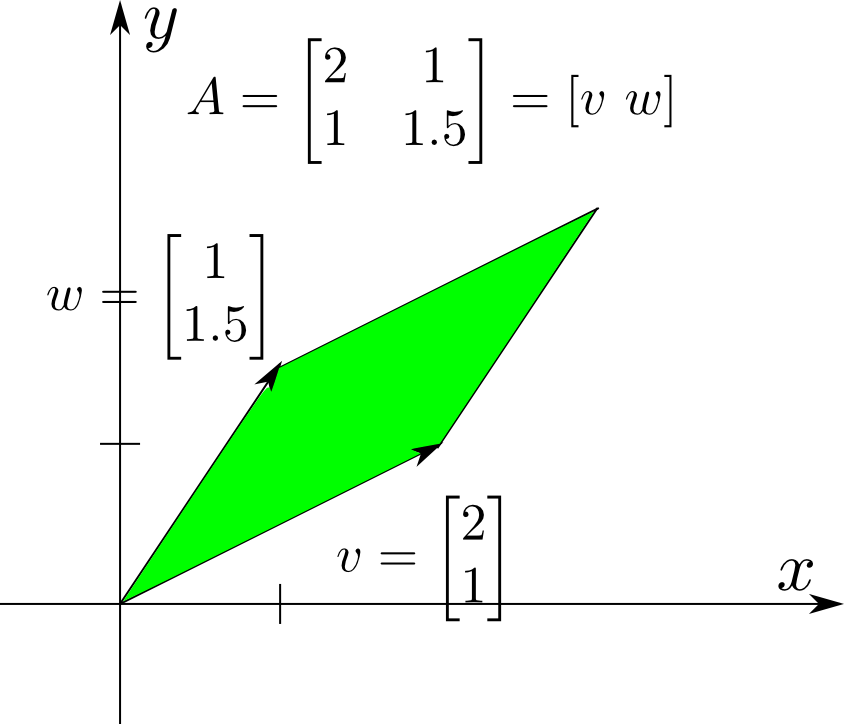
\includegraphics[width=0.8\textwidth]{FIGURES/detgraphic}  
       \end{center}
       \begin{itemize}
       \item    Area of the green parallelogram spanned by $v$ and $w$    
         $$
         \det A = 2\times 1.5 - 1\times 1 = 2
         $$
       \end{itemize}
     \end{column}
     \begin{column}{0.5\textwidth}
       \begin{itemize}
       \item Order of vectors matters
      $$
       det
       \begin{bmatrix}
         b & a\\ d & c
       \end{bmatrix}
       = - \det
       \begin{bmatrix}
         a & b\\ c & d
       \end{bmatrix}
       $$
     \item $\det [w\,\, v] = -\det[v\,\, w]$.
       Reversing the orientation changes the sign
     \item if $v = \lambda w$: parallelogram is flat, area is 0.
       $$
       \det
       \begin{bmatrix}
         a & \lambda a \\b &\lambda b
       \end{bmatrix}
       = \lambda a b - \lambda a b = 0.
       $$
     \item A matrix with null determinant is \myemph{singular}.
     \item Important rule  \fbox{$det(AB) = \det(BA) = \det(A)\det(B)$}
       Note that $\det(A+B) \not= \det(A) + \det(B)$
       \end{itemize}
      \end{column}
  \end{columns}
\end{frame}
\begin{frame}
  \frametitle{In 3D}
  \begin{columns}
    \begin{column}{0.4\textwidth}
      \begin{center}
        
\includegraphics[width=0.9\textwidth]{FIGURES/parallelepided}  
      \end{center}
       $$\det
      \begin{bmatrix}
        a_1 & b_1 & c_1\\
        a_2 & b_2 & c_2\\
        a_3 & b_3 & c_3\\
      \end{bmatrix}=
      $$
      $
      a_1 b_2 c_3 + a_2 b_3 c_1 + a_3 b_1 c_2 -a_2 b_1 c_3 -a_1 b_3 c_2 -a_3 b_2 c_1
      $
    \end{column}
    \begin{column}{0.6\textwidth}
      \begin{itemize}
      \item  $v_1 =
      \begin{bmatrix}
        a_1\\a_2\\a_3
      \end{bmatrix},
      v_2 =
      \begin{bmatrix}
        b_1\\b_2\\b_3
      \end{bmatrix}
      ,v_3 =
      \begin{bmatrix}
        c_1\\c_2\\c_3
      \end{bmatrix}$
    \item
      $\det
      \begin{bmatrix}
        a_1 & b_1 & c_1\\
        a_2 & b_2 & c_2\\
        a_3 & b_3 & c_3\\
      \end{bmatrix}
      = \det [v_1, v_2, v_3]
      $
      \item Volume of the parallelepiped spanned by $v_1$, $v_2$ and $v_3$.
      \item Order of the vectors counts!
      \item If one vector is combination of the others: parallepiped flat, volume is 0.
      \item Matlab \texttt{det} command! - Python Numpy has a similar one (in linalg module). Not limited to 3x3 matrices.
      \end{itemize}
    \end{column}
  \end{columns}
\end{frame}


\begin{frame}{Exercises}
  Pen and paper.
  \begin{itemize}
  \item Compute the products $AB$ and $BA$ for the following matrices
    $$A =
    \begin{pmatrix}
      2 & 1\\
      4 & 2\\
    \end{pmatrix},\quad
    B =
    \begin{pmatrix}
      1 & -2\\
      -2 & 4
    \end{pmatrix}
    $$
  \item Compute their determinant and traces.
  \end{itemize}
  With numpy.
  \begin{itemize}
  \item  $numpy.linalg$ subpackage has functions for trace and determinants.
  \item Find them and play with the two matrices above.
  \end{itemize}
 
\end{frame}

\begin{frame}
  \frametitle{Inverse Matrices}
  \begin{itemize}
  \item $A =
    \begin{bmatrix}
      1 & 3\\ 2 & 7
    \end{bmatrix}
    $,
    $B =
    \begin{bmatrix}
    7 & -3 \\
    -2 & 1
    \end{bmatrix}
    $
    $$
    AB =
    \begin{bmatrix}
      1 & 0 \\0 & 1
    \end{bmatrix} = I,\quad BA =
    \begin{bmatrix}
      1 & 0\\
      0 & 1
    \end{bmatrix}
    = I
    $$
    $A$ and $B$ are \myemph{inverse} of each other: $A = B^{-1}$, $B = A^{-1}$.
  \item $A$ is \myemph{invertible} iff $\det(A) \not= 0$.
  \item Example: system of equations
    $$
    \begin{cases}
      3x + 2y &=5\\
      2x + y &=-1
    \end{cases}\,\text{ in matrix form:}\,
    \udesc{\det=3-4 = -1\not=0}{\odesc{C}{
    \begin{bmatrix}
      3 & 2\\ 2 & 1
    \end{bmatrix}}}
    \begin{bmatrix}
      x \\ y
    \end{bmatrix}=
    \begin{bmatrix}
      5 \\ -1
    \end{bmatrix}
    $$
  \item Solution
    $$
    C^{-1} =
    \begin{bmatrix}
      -1 & 2\\2 & -3
    \end{bmatrix},\quad
    C^{-1}C
    \begin{bmatrix}
      x\\y  
    \end{bmatrix} = 
    I
    \begin{bmatrix}
      x\\y
    \end{bmatrix}
    =
    \begin{bmatrix}
      x \\ y
    \end{bmatrix}
    =
    C^{-1}
    \begin{bmatrix}
      5\\-1
    \end{bmatrix} =
    \begin{bmatrix}
      -7\\13
    \end{bmatrix}
    $$
  \item Matlab and Python-numpy have functions to invert matrices and solve linear systems.
  \end{itemize}
\end{frame}




\begin{exercise}
  \begin{itemize}
  \item Pen and paper. Let $C$ be the matrix
    $$
    \begin{pmatrix}
      1 & 3\\
      2 & 8
    \end{pmatrix}
    $$
  \item Compute its inverse by writing
    $$
    \begin{pmatrix}
      1 & 0\\
      0 & 1
    \end{pmatrix} =
    C
    \begin{pmatrix}
      a & b\\
      c & d
    \end{pmatrix}
    =
    \begin{pmatrix}
      a + 3c & b + 3d\\
      2a + 8c& 3b + 8d
    \end{pmatrix}
    $$
  \item Explain why. There is a linear system to solve. Can you?
  \item Try with Python and the \texttt{numpy.linalg.inv()} function.
  \end{itemize}
\end{exercise}

\begin{frame}
  \frametitle{For Non-Square-Matrices}
  \begin{itemize}
  \item Notions of right-inverse or left inverses.
  \item General construction of the Moore-Penrose
    Pseudo-Inverse. Works both with matrices with more lines than
    columns -- \myemph{overdetermined linear systems} and the
    opposite: less lines than columns -- \myemph{underdetermined
      linear systems}.
  \item \texttt{pinv} function in Matlab, \texttt{pinv} function in \texttt{numpy.linalg} python package.
  \item Intimately connected to \myemph{linear least-squares problems} and the \myemph{Singular Value Decomposition}.
  \item In turn intimately connected to eigenvalues and eigenvectors problems (spectral theory) for square matrices.
  \end{itemize}
\end{frame}

\section{Linear Mappings}


\begin{frame}
  \frametitle{Linear Mapping}
  \begin{itemize}
  \item Mapping between vectors with only addition of coordinates, multiplications by scalar and no constant terms.
  \item Example
    $$
    f
    \begin{bmatrix}
      x\\y\\z
    \end{bmatrix}
    =
    \begin{bmatrix}
      x+3y\\z-2x
    \end{bmatrix}
    $$
  \item Non linear example
    $$g
    \begin{bmatrix}
      x\\y\\z
    \end{bmatrix}
    =
    \begin{bmatrix}
      x^2+3yz\\z-2x^2 + 1
    \end{bmatrix}
    $$
    There are powers and constant terms.
  \end{itemize}
\end{frame}

\begin{frame}
  \frametitle{Linearity}
  \begin{itemize}
  \item This means $f(v+ \lambda v') = f(v) + \lambda f(v')$
    \begin{align*}
     f\left(
    \begin{bmatrix}
      x\\y\\z
    \end{bmatrix}+\lambda
    \begin{bmatrix}
      x'\\y'\\z'
    \end{bmatrix}
    \right)
    &= f
    \begin{bmatrix}
      x+\lambda x'\\y+\lambda y'\\z+\lambda z'
    \end{bmatrix}\\
    &=
    \begin{bmatrix}
      x+\lambda x'+3(y+\lambda y')\\
      z+\lambda z'-2(x+\lambda x')
    \end{bmatrix}\\
    &=
    \begin{bmatrix}
      x+3y\\
      z-2x\\
    \end{bmatrix}
    +\lambda 
    \begin{bmatrix}
      x'+3y'\\
      z'-2x'
    \end{bmatrix}\\
    &= f
    \begin{bmatrix}
      x\\y\\z
    \end{bmatrix}
    + \lambda f
    \begin{bmatrix}
      x'\\y'\\z'
    \end{bmatrix}
  \end{align*}
\item $f$ is linear.
\end{itemize}
\end{frame}



\begin{frame}
  \begin{itemize}
  \item Example: Compute the product of 
    $$
    A =
    \begin{bmatrix}
        1 & 3 & 0\\
      -2 & 0 & 1
    \end{bmatrix}\text{ and }
    v =
    \begin{bmatrix}
      x\\y\\z
    \end{bmatrix}
    $$
    \pause
  \item We find precisely the value of 
    $$   
    f
    \begin{bmatrix}
      x\\y\\z
    \end{bmatrix}
    =
    \begin{bmatrix}
      x+3y\\-2x+z
    \end{bmatrix}=
    \begin{bmatrix}
      x+3y\\z-2x
    \end{bmatrix}
    $$
  \item Each linear mapping can be written that way. Often use the same notation for the matrix and the linear mapping.
  \end{itemize}
\end{frame}



\begin{frame}
  \frametitle{Matrices /linear mappings as geometric transformations}. 
  \begin{columns}
    \column{0.5\textwidth}
    \begin{center}
    Projection  on $x-y$ plane
    \end{center}
    \column{0.5\textwidth}
    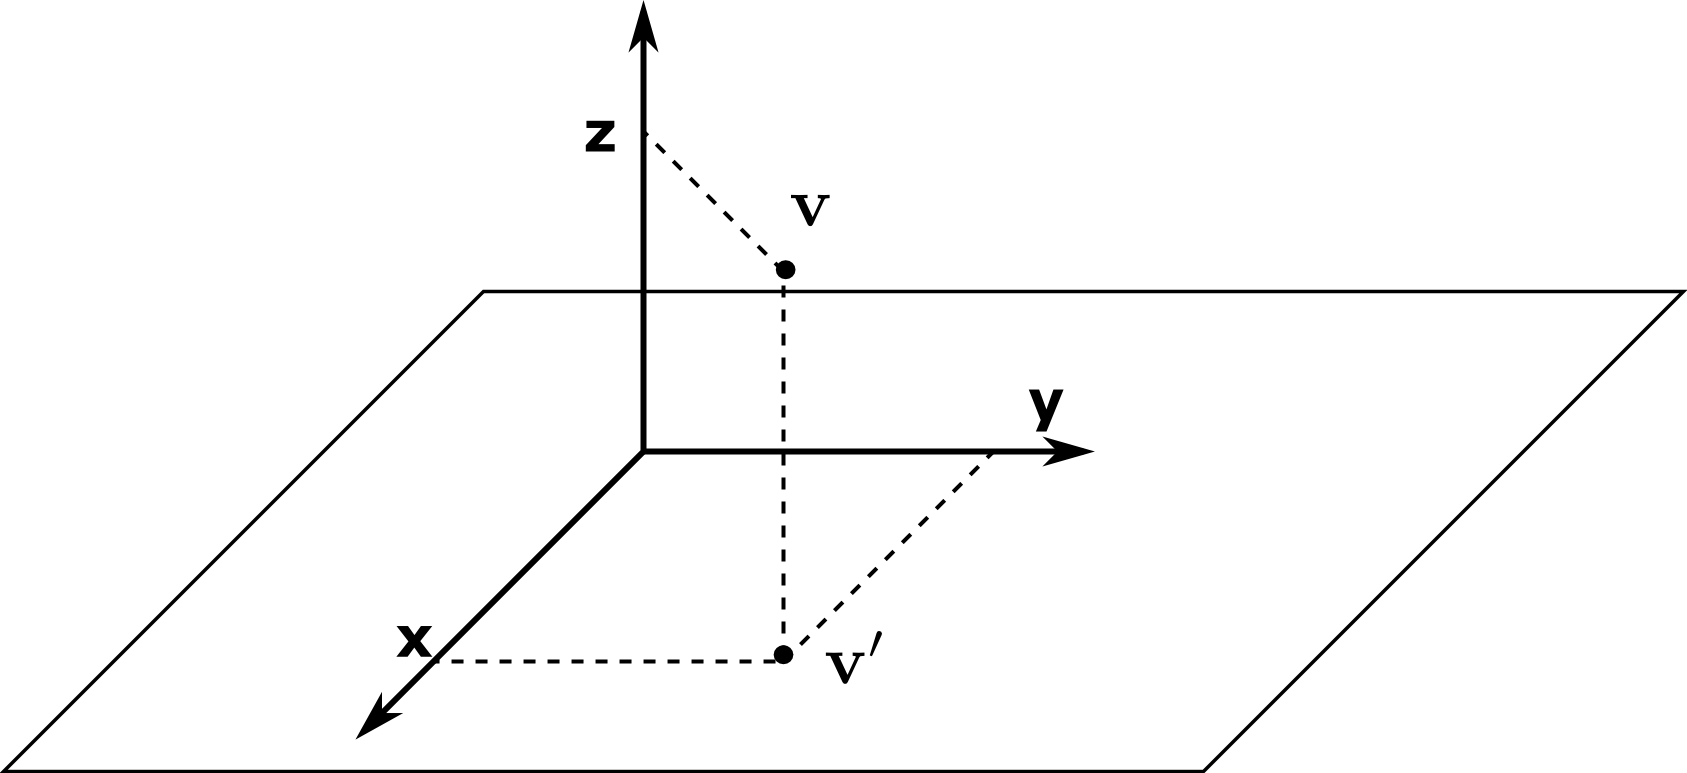
\includegraphics[width=\textwidth]{FIGURES/3dto2dproj}
  \end{columns}
  \begin{center}
    \includegraphics[width=0.9\textwidth]{FIGURES/simpletransforms}\\
    Rotation of angle $\theta$ \hfill anisotropic scaling \hfill ~~~~~~shear~~~~~~~~~~~
  \end{center}
\end{frame}

\begin{frame}
  \begin{itemize}
  \item projection $\RR^3\to\RR^2$
    $$
    F
    \begin{bmatrix}
      x \\y \\z
    \end{bmatrix}
    =
    \begin{bmatrix}
      x \\y
    \end{bmatrix},\quad F =
    \begin{bmatrix}
      1 & 0 & 0\\
      0 & 1 & 0\\
      0 & 0 & 0
    \end{bmatrix}
    $$
  \item Rotation of angle $\theta$ from $\RR^2\to\RR^2$:
    $$
    R_\theta
    \begin{bmatrix}
      x \\y
    \end{bmatrix}
    =
    \begin{bmatrix}
      x\cos\theta - y\sin\theta\\
      x\sin\theta + y\cos\theta
    \end{bmatrix},\quad
    R_\theta =
    \begin{bmatrix}
      \cos\theta & -\sin\theta\\
      \sin\theta & \cos\theta
    \end{bmatrix}
    $$
  \item Scaling by a factor $\alpha$ in $x$ and $\beta$ in $y$:
    $$
    S
    \begin{bmatrix}
     x\\y 
    \end{bmatrix}
    = 
    \begin{bmatrix}
      \alpha x\\
      \beta y
    \end{bmatrix},\quad
    S =
    \begin{bmatrix}
      \alpha & 0\\0 & \beta
    \end{bmatrix}
    $$
  \item Shear of the $y$-axis with  angle $\theta$:
    $$
    \Ss
    \begin{bmatrix}
      x\\y
    \end{bmatrix}
    =
    \begin{bmatrix}
      x + \sin\theta y\\
      y
    \end{bmatrix},\quad
    \Ss =
    \begin{bmatrix}
      1 &\sin\theta\\
      0 & 1
    \end{bmatrix}
    $$
  \end{itemize}
\end{frame}

\begin{frame}
  \frametitle{Eigenvalues/vectors of a Square Matrix}
  \begin{itemize}[<+->]
  \item $A =
    \begin{bmatrix}
      11 & 27\\ -4 & -10
    \end{bmatrix}
    $.~~~~~~ $A
    \begin{bmatrix}
      9\\-4
    \end{bmatrix}=
    \begin{bmatrix}
      -9\\4
    \end{bmatrix}$.~~~~~~
    $A
    \begin{bmatrix}
      -3\\1
    \end{bmatrix}
    =
    \begin{bmatrix}
      -6 \\ 2
    \end{bmatrix}
    $\vfill
  \item $A$ multiplies the vector $[-9, 4]^\top$ by -1 and multiplies the vector $[-3, 1]^\top$ by 2. If I take $v= [9\alpha, -4\alpha]^\top$, 
    $Av = -v$. If I take $w = [-3\beta,\beta]^\top$, $Aw = 2w$.\vfill
  \item $-1$ and $3$ are \myemph{\textsc{the} eigenvalues} of
    $A$. $[-9,4]^\top$ and $[-3,1]^\top$ are \myemph{\textsc{some}
      eigenvectors} of $A$ corresponding to these eigenvalues.\vfill
  \item $A$ acts as scaling by -1 in the direction of vector $[9,-4]^\top$ and by scaling by $2$ in the direction of vector $[-3,1]^\top$.\vfill
  \item Any vector of $\RR^2$ can be written as $\alpha [9,-4]^\top + \beta [-3,1]^\top$. Action of $A$:
    $$
    A\left(\alpha [9,-4]^\top + \beta [-3,1]^\top\right) = -\alpha[9,-4]^\top + 2\beta[-3,1]^\top.
    $$
  \end{itemize}
\end{frame}


\begin{frame}
  \frametitle{Case of Symmetric Matrices}
  \begin{itemize}
  \item Eigenvectors for different eigenvalues are orthogonal. Can be chosen with norm 1.
  \item Eigenvectors + eigenvalues: Linear``elliptic--like'' scaling.
  \end{itemize}
  \begin{center}
    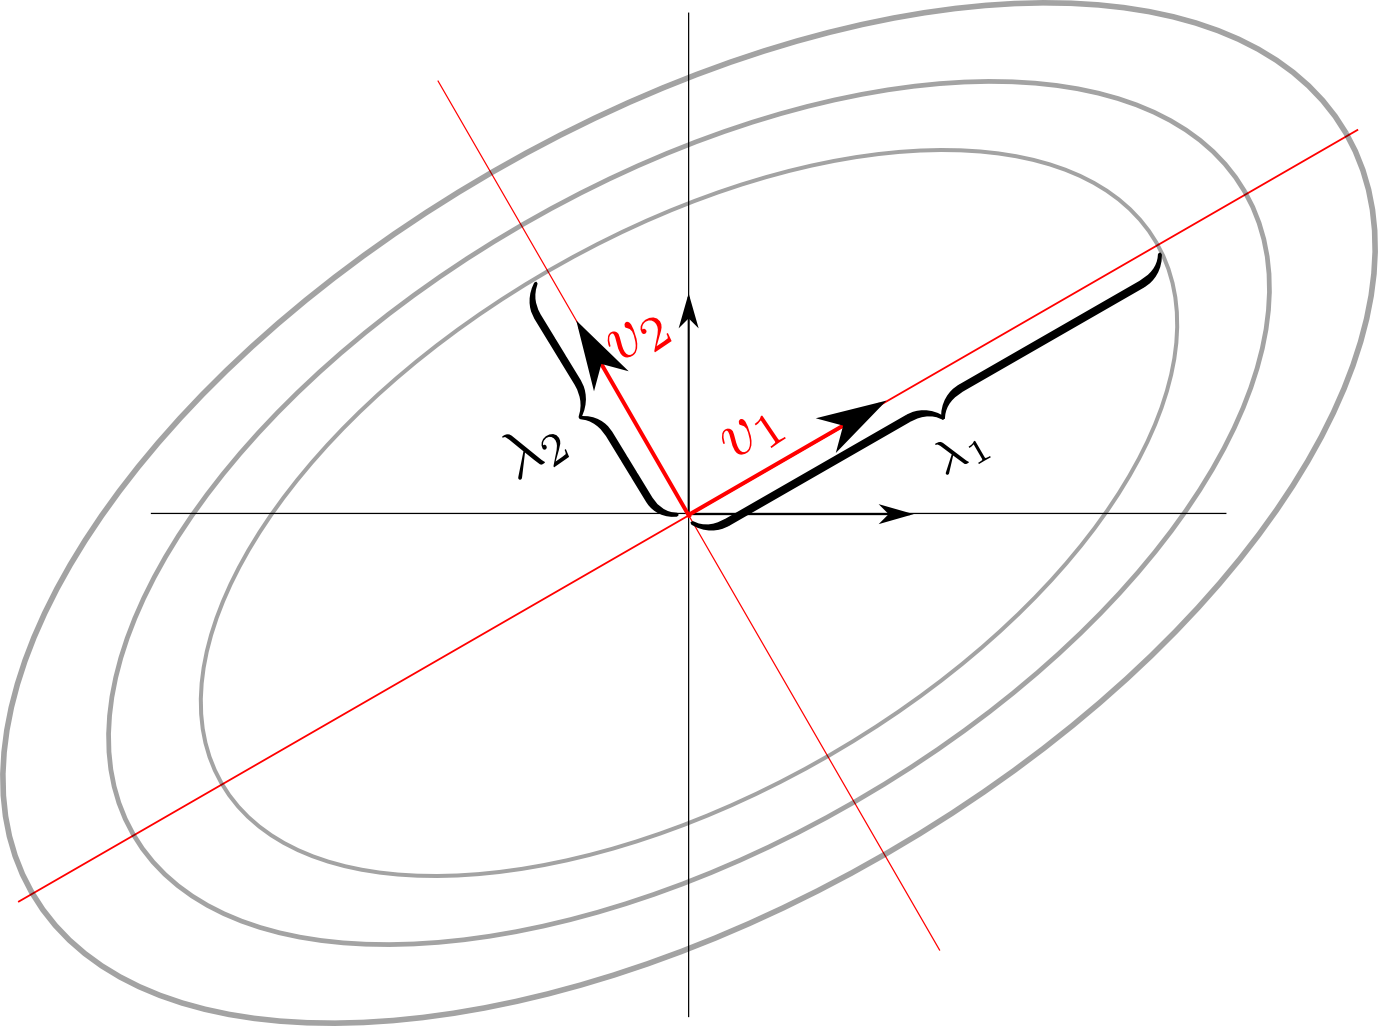
\includegraphics[width=0.5\textwidth]{FIGURES/eigssymm}
  \end{center}
  \begin{itemize}
  \item Can be interpreted as ``Rotate, scale in each axis direction, then rotate back''.
  \end{itemize}
\end{frame}

\begin{frame}
  \frametitle{Matrix Rank}
  \begin{itemize}
  \item Linear mapping $f:\RR^n \to \RR^m$, $A$ matrix associated. \myemph{Rank} of $A$ = dimension of the image of $f$, i.e. dimension of the 
    set made of the $f(x_1,\dots,x_n)$.
  \item Rank of projection $F$ above: 2: all vectors of $\RR^3$ are projected on the plan of vectors $[x,y,0]^T$.
  \item Take $A =
    \begin{bmatrix}
      1 & 2\\
      2 & 4\\
    \end{bmatrix}
    $. $A$ has rank 1. 
    $$
    f(x,y) =  \begin{bmatrix}
      1 & 2\\
      2 & 4\\
    \end{bmatrix}
    \begin{bmatrix}
      x\\y
    \end{bmatrix}
    =
    \begin{bmatrix}
      x + 2y\\
      2x + 4y
    \end{bmatrix}
    $$
    All the values of $f$ belong to the line $y = 2x$, dimension 1 subspace of $\RR^2$.
  \item The square matrix $A$, says size $n\times n$, is invertible is its rank is $n$.
  \item For a square matrix, its rank is the number of non-zeros eigenvalues.
  \end{itemize}
\end{frame}



\begin{frame}
  \frametitle{Meaning of the Product}
  \begin{itemize}
  \item $M$ and $N$ the linear mappings $
    \begin{bmatrix}
      2 & 2\\
      1 & 3\\
      1 & -1\\
    \end{bmatrix}
    $ and 
    $
    \begin{bmatrix}
      1 & 3 & 0\\
      -2 & 0 & 1
    \end{bmatrix}
    $
  \item
    Apply $N$ to $
    \bv = \begin{bmatrix}
      x \\ y \\ z
    \end{bmatrix}
    $
    and $M$ to the result:
    $$
    N \bv = \begin{bmatrix}
      1 & 3 & 0\\
      -2 & 0 & 1
    \end{bmatrix}\begin{bmatrix}
      x \\ y \\ z
    \end{bmatrix}
    = 
    \begin{bmatrix}
      x + 3y\\
      -2x + z
    \end{bmatrix}
    $$
    \item and{\small
      $$
      \begin{bmatrix}
      2 & 2\\
      1 & 3\\
      1 & -1\\
    \end{bmatrix}
     \begin{bmatrix}
      x + 3y\\
      -2x + z
    \end{bmatrix}
    =\onslide<2->
    \begin{bmatrix}
      -2x+6y+2z\\
      -5x + 3y+3z\\
      3x + 3y-z
    \end{bmatrix}
    =\onslide<3->
    \begin{bmatrix}
      -2 & 6 & 2\\      -5 & 3 & 3\\
      3 & 3 & -1
    \end{bmatrix}
    \begin{bmatrix}
      x\\y\\z
    \end{bmatrix}
    $$}
    % \item VIP (Very Important Property) \myemph{Matrix multiplication correspomds to chaining linear transforms}!
  \end{itemize}
\end{frame}





\begin{frame}
  \frametitle{Matrix Product as Chain Application of Linear Mappings}
  \begin{itemize}
  \item We found that 
    $$
    M\left (N\bv\right) = \udesc{\text{Matrix product}}{M N}\bv
    $$
  \item Very Important Property: Matrix product corresponds to chain application (composition) of linear mappings!
  \end{itemize}
\end{frame}

\begin{frame}
  \frametitle{So far}
  \begin{itemize}
  \item We talked of vectors, vector spaces, dimension, inner products
  \item Matrices, operations on them, transposition, product of matrices,
    \item Square matrices and their algebra, symmetric matrices, Traces, determinants.
    \item linear mappings, ranks, eigenvalues/vectors.
    \item matrix products and composition of linear mappings.
  \end{itemize}
\vfill
  \begin{center}
    \large
    Read the Linear Algebra Tutorial and Reference on Absalon!\\
    Next time: pencil and paper for manual computations of convolutions!
  \end{center}
  This will also be useful for other courses!
\end{frame}



\end{document}


